\documentclass{standalone}
\usepackage{tikz}
\usepackage{tikz-qtree}
\usepackage{xcolor}
\usetikzlibrary{arrows}
\usepackage{fontspec}
\setmainfont{Helvetica}
\begin{document}
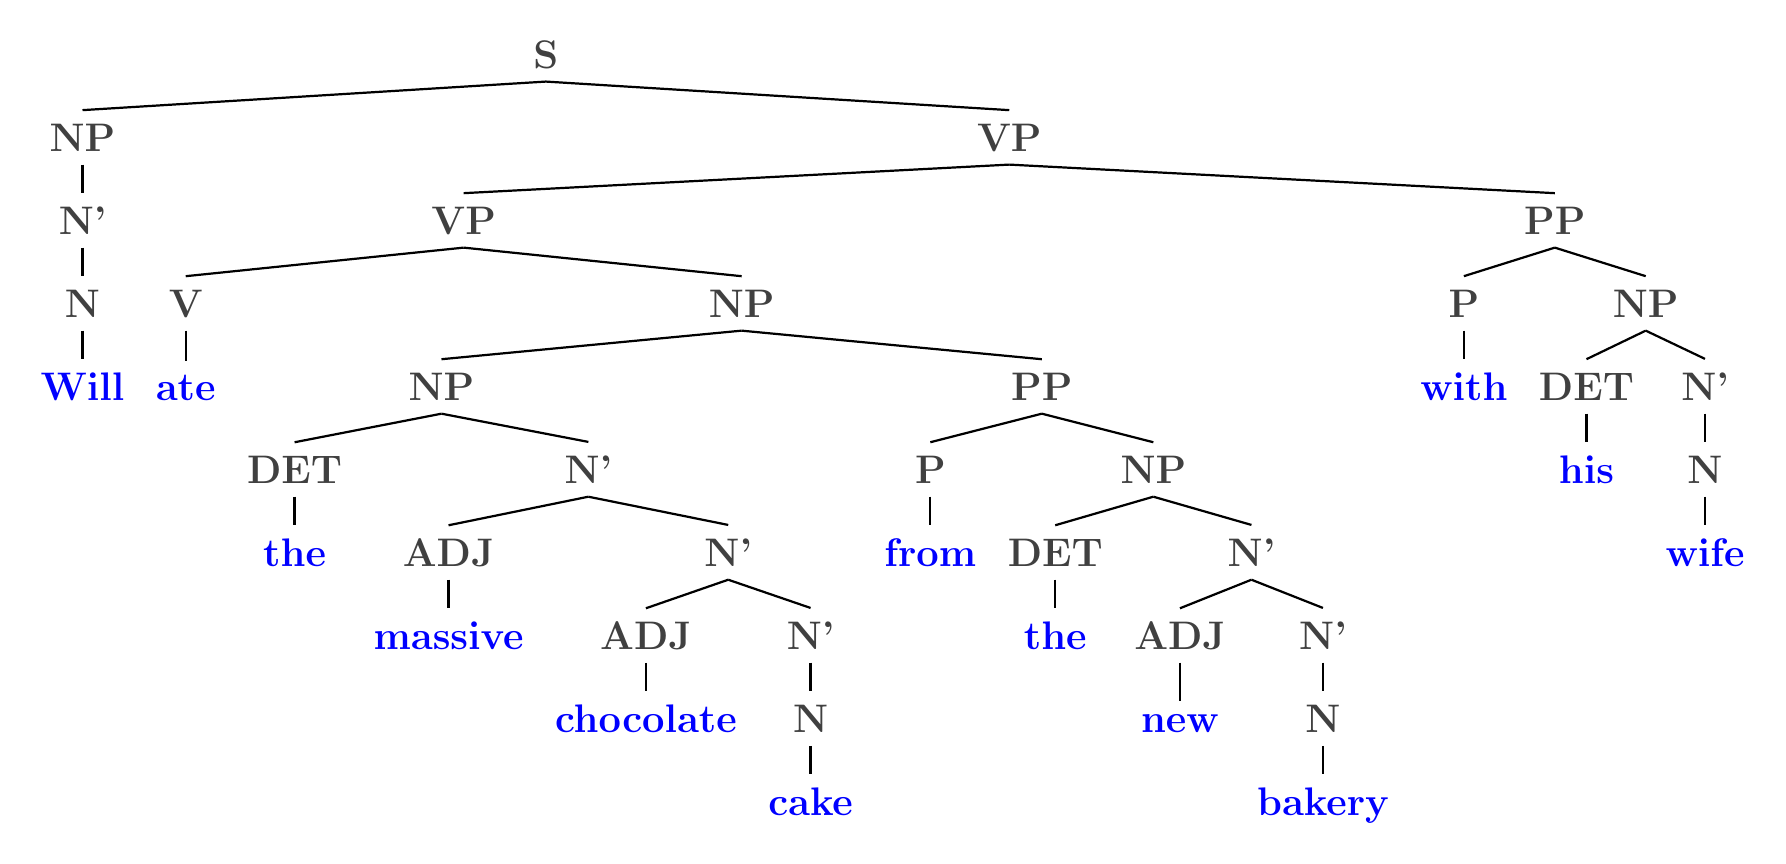
\begin{tikzpicture}
\tikzset{level distance=30pt}
\tikzset{every  leaf node/.style={text=blue,font=\bf}}
\tikzset{every internal node/.style={text=darkgray,font=\bf}}
\tikzset{edge from parent/.append style={thick}}

\Large

\Tree[.S [.NP [.N' [.N Will ] ] ] [.VP [.VP [.V ate ] [.NP [.NP [.DET the ] [.N' [.ADJ massive ] [.N' [.ADJ chocolate ] [.N' [.N cake ] ] ] ] ] [.PP [.P from ][.NP [.DET the ] [.N' [.ADJ new ] [.N' [.N bakery ] ] ] ] ] ] ][.PP [.P with ] [.NP [.DET his ] [.N' [.N wife ] ] ] ] ] ]


\end{tikzpicture}
\end{document}
